\chapter{Introduction}
\label{ch:Introduction}

When rumours of a novel respiratory virus, which would later be dubbed coronavirus disease 2019, or short COVID-19, first emerged from the People's Republic of China in late 2019, there was a lot of uncertainty regarding its danger potential. Authorities were hesitant to acknowledge the threat of a possible epidemic, and people were discouraged from stocking up on equipment such as protective face masks. When the virus spread to other countries across the globe and its impact could no longer be ignored, governments reversed course and imposed various restrictions on their respective populations, even going as far as sending a whole country into lockdown, in order to halt, or at least slow the spread of the virus. However, the sheer number of cases soon threatened to overwhelm healthcare systems worldwide.

In order to prevent this worst-case scenario, it became paramount to identify sources of infection and interrupt transmission chains. The efficient tracing of infected individuals' social contacts plays an integral part in preventing the spreading of a disease, and had been a well-established procedure well before the emergence of COVID-19, where for instance a verified case of tuberculosis requires a notification of the health departments \cite{enwiki_1097839709}. This is done to isolate persons who might have been infected by or have themselves been the source of infection of the individual, and therefore interrupt the transmission chain early, comparable to removing a domino piece to stop the fall of subsequent ones.

Most attention regarding science during the pandemic has focused on the medical field, especially the research of effective vaccines and treatments against the virus, but also virological factors (e.g. which individual features would predispose someone to infection and/or a severe course of illness, how the virus is transmitted from person to person, etc.). Now that the pandemic has mostly passed, a retrospective view suggests that there were no comprehensive insights into infection dynamics on a societal level, as evidenced by the at times incoherent measures taken in order to combat the spread of the virus.

It is therefore necessary to establish a set of methods to effectively and efficiently analyse the social aspects of viral transmission and spread in order to be better prepared for a similar situation in the future. In the recent months, more work tackling this topic has emerged, and the field of computational social sciences offers a wide array of tools to address this problem.

Computational Social Science (CSS) is an interdisciplinary field that uses advanced computa-tional methods to investigate social phenomena and human behavior. It combines elements of social sciences, such as sociology, economics, and psychology, with data science, computer science, and statistics. The aim is to glean insights into the complex dynamics of human societies through analysis of big data, modeling, and simulations, typically drawing from data sources like social media, web pages, or even administrative records.

The essence of CSS is the quantification and analysis of social phenomena, facilitating a deeper understanding of individual and group behaviors, social structures, and societal trends. By leveraging computational tools such as machine learning, network analysis, natural language processing, and agent-based modeling, CSS allows researchers to explore questions that were previously inaccessible due to the sheer complexity of the social systems involved. This often involves handling large and complex datasets, managing issues of privacy and ethics, and interpreting results in a meaningful social context.

\section{Contact Tracing}
\label{sec:contact_tracing}

Many contact tracing initiatives were established during the course of the pandemic in most developed countries, e.g. automatic tracing via mobile apps; although they differ in the level of detail that was (or still is) being recorded, data collected at least included the source of infection, i.e. a symptomatic or, once tests had become widely available, positively tested patient, and said patient's social contacts, i.e. the people who had come into contact with them, and who thus could have been infected themselves and possibly spread the virus further. More rigorous systems also recorded covariates such as age, job or co-morbidities, which may play a role in transmission. 

A dataset consisting of records of the form (source, contact) can be modelled as a social network, a concept derived from graph theory, where individuals constitute a set of vertices, and contacts between individuals are represented by edges between the respective vertices; for an illustration, refer to figure \ref{fig:example_case_network}. These networks can be efficiently analysed using methods stemming from the field of computer science; thus, it becomes possible to identify dynamics in the spread of the virus on a social level, which are traditionally overlooked in virology. Common network effects include betweenness centrality, a measure for how instrumental a person is in facilitating the viral spread, or community detection and shortest paths lengths to determine whether infections emerge in clusters. Additionally, if further covariates like age, pre-existing illness or profession were also collected during the contact tracing procedure, methods from the field of data science can reliably discover patterns in the data and thus identify covariates that influence transmission, e.g. whether younger people are more likely to get infected and/or infect others compared to other age groups.

\begin{figure}
	\begin{mdframed}
		\centering
		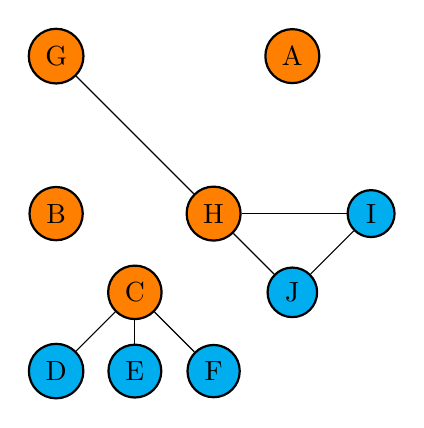
\begin{tikzpicture}
		\begin{scope}[every node/.style={circle,thick,draw,fill=orange}]
			\node (A) at (2,2) {A};
			\node (B) at (-1,0) {B};
			\node (G) at (-1,2) {G};
			\node (C) at (0,-1) {C};
			\node (H) at (1,0) {H};
		\end{scope}
		
		\begin{scope}[every node/.style={circle,thick,draw,fill=cyan}]
			\node (D) at (-1,-2) {D};
			\node (E) at (0,-2) {E};
			\node (F) at (1,-2) {F};
			\node (I) at (3,0) {I};
			\node (J) at (2,-1) {J};
		\end{scope}
		
		\begin{scope}
			\path (C) edge node {} (D);
			\path (C) edge node {} (E);
			\path (C) edge node {} (F);
			\path (G) edge node {} (H);
			\path (H) edge node {} (I);
			\path (H) edge node {} (J);
			\path (I) edge node {} (J);
		\end{scope}
	\end{tikzpicture}
	\caption{Exemplary case contact network. Confirmed cases are coloured orange, and reported contacts are coloured cyan. This network contains four connected components: $\{\{A\},\{B\},\{C,D,E,F\},\{G,H,I,J\}\}$}
	\label{fig:example_case_network}
	\end{mdframed}
\end{figure}

\section{Relational Event Models}
\label{sec:intro_rem}

These static networks, however, can only give a partial representation of reality, since temporal information is omitted; thus, it is assumed that all infections and contact nominations happen simultaneously, whereas in reality, events occur sequentially. Therefore, infected patient $A$ might name person $B$ as a contact at time $t_1$, and $B$ might himself be recorded as a patient at a later time $t_2$, nominate persons $C,D$ as contacts, and so on. Obviously, this temporal aspect leads to a range of additional possible effects. Do dyads (pairs of source, contact) appear repeatedly (repetition), is a person $B$ who gets nominated as a contact by $A$ at time $t_n$ more likely to become a patient, and nominate $A$ in return at a later time $t_{n+m}$ (reciprocation), or is there a tendency for cyclic closure, where $A$ nominates $B$, $B$ then nominates $C$, and $C$ nominates $A$?

A common method for modelling time-stamped relational data of the form (time, source, target) are Relational Event Models, short REM, which were first proposed by \cite{butts20084}. They will be discussed further in chapter \ref{ch:methods}.

\section{Relational Hyperevent Models}
\label{sec:intro_rhem}

An obvious shortcoming of relational event models is their dyadic nature, i.e. their inherent assumption that all interactions only involve two people at a time. Of course, this is not an accurate representation of reality. Think, for example, of John sending an email addressed at multiple of his colleagues, or in the context of COVID, Jane testing positive after attending a party and naming all the other guests as contacts. Some workarounds have been proposed to tackle this problem, like treating all interactions separately, or grouping all receiver nodes (email recipients and party attendees in our examples, respectively) into a single node. Refer to figure \ref{fig:polyadic_interactions} for an illustration. The problem with the former method is the fact that is treats the interactions as independent, while the latter may be unfeasible or even intractable for large datasets.

\begin{figure}
	\begin{mdframed}
		\centering
		\begin{subfigure}[t]{0.45\linewidth}
			\vskip 0pt
			\centering
			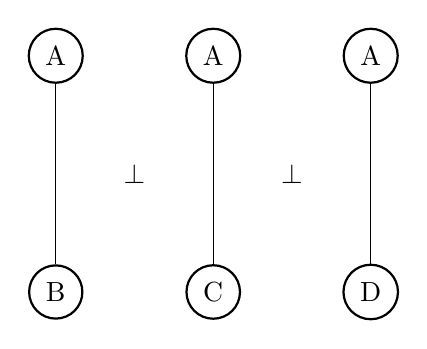
\begin{tikzpicture}
				\begin{scope}[every node/.style={circle,thick,draw}]
					\node (A1) at (0,0) {A};
					\node (A2) at (2,0) {A};
					\node (A3) at (4,0) {A};
					\node (B) at (0,-3) {B};
					\node (C) at (2,-3) {C};
					\node (D) at (4,-3) {D};
				\end{scope}
				
				\begin{scope}
					\node[draw=none] (A1A2) at (1,0) {};
					\node[draw=none] (BC) at (1,-3) {};
					\node[draw=none] (A2A3) at (3,0) {};
					\node[draw=none] (CD) at (3,-3) {};
				\end{scope}
				
				\begin{scope}
					\path (A1) edge node {} (B);
					\path (A2) edge node {} (C);
					\path (A3) edge node {} (D);
					\path (A1A2) edge[draw=none] node {$\perp$} (BC);
					\path (A2A3) edge[draw=none] node {$\perp$} (CD);
				\end{scope}
			\end{tikzpicture}
			\caption{Method 1: Model one edge for each node of the receiver set. Edges are assumed to be independent.}
		\end{subfigure}
		\hfill
		\begin{subfigure}[t]{0.45\linewidth}
			\vskip 0pt
			\centering
			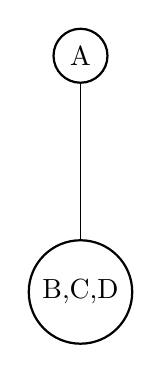
\begin{tikzpicture}
				\begin{scope}[every node/.style={circle,thick,draw}]
					\node (A) at (0,0) {A};
					\node (B) at (0,-3) {B,C,D};
				\end{scope}
				
				\begin{scope}
					\path (A) edge node {} (B);
				\end{scope}
			\end{tikzpicture}
			\caption{Method 2: Model receiver set as a single node}
		\end{subfigure}
	\caption{Two ways to approximate polydiadic interactions. In this example, $A$ has an interaction with $B, C,$ and $D$ at the same time (e.g. They meet for a drink at the pub and $A$ subsequently falls ill with Coronavirus).}
	\label{fig:polyadic_interactions}
	\end{mdframed}
\end{figure}

To address these issues, an extension to REM, named Relational Hyperevent Models, short RHEM, has been proposed by \cite{lerner2019rem}. These models use hyperedges instead of the regular, dyadic edges known from graph theory; each hyperedge consists of a sender (e.g. a positively tested patient) and a set of receivers (e.g. attendees of a birthday party). These models can be used to discover effects in a fashion similar to REM, but with additional effects specific to polyadic interactions like partial repetition, where the receiver set is only partially the same in a repeated interaction (e.g. John plays tennis with Jane and Max, gets ill and nominates Max and Jane at time $t_n$, and again gets sick after grabbing coffee with Jane and Peter at time $t_{n+m}$ and thereafter nominates them), or unordered repetition, where an interaction is repeated involving the same actors, but the direction is not the same (e.g. reaching back to the previous example, John, Jane and Max again meet for tennis, whereafter Jane tests positive and nominates John and Max as contacts at time $t_{n+m}$). These RHEM will likewise be discussed in chapter \ref{ch:methods} in more detail.

\section{Goal}
\label{sec:intro_goal}

This work's primary aim is to review three different methods that have been proposed for analysing COVID-19 case contact networks, namely Social Network Analysis (SNA), Relational Event Models (REM) and Relational Hyperevent Models (RHEM). This review process will consist of an investigation of reproducibility of previously reported results through the usage of equivalent methodology, and a comparison of results between these three methods. To this end, SNA, REM and RHEM will be used to analyse five (six) distinct case contact networks. Results of these analyses are then compared horizontally, i.e. between datasets, and vertically, i.e. between methods. Chapter \ref{ch:previous_work_data} will present and briefly discuss the research and data upon which this work relies and builds. Chapter \ref{ch:methods} will recapitulate the theoretical fundamentals of SNA, REM and RHEM and outline how these methods are applied to the data. Analysis results will be presented and discussed in chapter \ref{ch:results_discussion}. Finally, chapter \ref{ch:outlook} will give an outlook on possible future extensions of this work.